\pdfminorversion=4
\documentclass[aspectratio=169]{beamer}

\mode<presentation>
{\usetheme{metropolis}
%\usecolortheme{spruce}
\usecolortheme{default}
}
%\setbeamertemplate{headline}{}
  %\setbeamercovered{transparent}
  %\expandafter\def\expandafter\insertshorttitle\expandafter{%
  %\insertshorttitle\hfill%
  %\insertframenumber\,/\,\inserttotalframenumber}
%}



%\usepackage[T2A]{fontenc}
\usepackage[utf8]{inputenc}
\usepackage[english, russian]{babel}

\usepackage{times}
\usepackage{amsthm}
\usepackage{graphicx}
\usepackage{subfigure}
\usepackage[mathscr]{eucal}
\usepackage{longtable}
\usepackage[all]{xy}
\usepackage{color}
\usepackage{colortbl}
\usepackage{multirow}
\usepackage{wrapfig}
\usepackage{ragged2e}
\usepackage{epstopdf}
\usepackage{lmodern}

\usepackage{tempora}


\usepackage{animate}

\usepackage{minted}

\usepackage{listings}
%\lstset{language=bash,keywordstyle={\bfseries \color{blue}}}

\usepackage[]{xcolor}

\definecolor{indigo}{rgb}{0.0, 0.25, 0.42}
\definecolor{arsenic}{rgb}{0.23, 0.27, 0.29}
\definecolor{bluegray}{rgb}{0.4, 0.6, 0.8}
\definecolor{cadet}{rgb}{0.33, 0.41, 0.47}
\definecolor{charcoal}{rgb}{0.21, 0.27, 0.31}
\definecolor{glaucous}{rgb}{0.38, 0.51, 0.71}
\definecolor{airforceblue}{rgb}{0.36, 0.54, 0.66}
\definecolor{darkgreen}{rgb}{0.0, 0.2, 0.13}


\metroset{sectionpage=none, block=fill}

%\setbeamercolor{frametitle}{bg=charcoal,fg=white}
%\setbeamercolor{section in head/foot}{bg=Brown}
%\setbeamercolor{author in head/foot}{bg=Brown}
%\setbeamercolor{date in head/foot}{fg=Brown}

%\setbeamercolor{block title}{bg = airforceblue!80, fg=black}
%\setbeamercolor{block body}{bg=airforceblue!30}

\defbeamertemplate*{frametitle}{}{%
    \leavevmode%
    \hbox to \paperwidth{%
    \begin{beamercolorbox}[wd=\paperwidth,ht=2ex,dp=3pt,left]{frametitle}%
        \ \insertframetitle
    \end{beamercolorbox}}
}


\newcommand{\myurl}[1]{{\color{indigo}\url{#1}}}%

%%%%%%%%%%%% TITLE PAGE %%%%%%%%%%%%%%%%%%
\title[]{\bf Efficient use of a text editor for HDL coding}
%\author[]{S. Kohani, K. Nishimura, V. Shebalin$^*$}\institute[]{\inst{}
\author{V. Shebalin}
\institute{\inst{}
%Budker Institute of Nuclear Physics\\
{\textit {}}
}
\date[]{December 1,  2022}

%\pgfdeclareimage[height=2.5cm]{mylogo}{Belle-logo.eps}
%%%%%%%%%%%%%%%%%%%%%%%%%%%%%%%%%%%%%%%%%%%



\begin{document}

%%%%%%%%%%%%%%%%%%%%%%%%%%%%%%%%%%%%%%%%%%%%%%%%%%%%
% TITLE PAGE
%%%%%%%%%%%%%%%%%%%%%%%%%%%%%%%%%%%%%%%%%%%%%%%%%%%%
\frame{\titlepage
%\centering \includegraphics[scale=0.3]{figs/uh.png}
}
%%%%%%%%%%%%%%%%%%%%%%%%%%%%%%%%%%%%%%%%%%%%%%%%%%%%

\footnotesize

%%%%%%%%%%%%%%%%%%%%%%%%%%%%%%%%%%%%%%%%%%%%%%%%%%%%
\section*{Editors}
%%%%%%%%%%%%%%%%%%%%%%%%%%%%%%%%%%%%%%%%%%%%%%%%%%%%
\begin{frame}{\secname}

  \begin{columns}
    \begin{column}{0.5\textwidth}
  \begin{itemize}
    \item {\bf Vim/NeoVim}
    \item {\bf VSCode} + TerosHDL
    \item {\bf Emacs} + verilog-mode/vhdl-mode
    \item {\bf Notepad++}, {\bf Sublime Text}, {\bf Eclipse}, ...
  \end{itemize}
      
    \end{column}
    \begin{column}{0.5\textwidth}
  \begin{block}{What we will be using}
    \begin{itemize}
      \item NeoVim + numerous plugins
      \item VSCode + TerosHDL + Python(Microsoft) \\
        see \myurl{https://terostechnology.github.io}
    \end{itemize}
    
  \end{block}
      
    \end{column}
  \end{columns}

\end{frame}
%%%%%%%%%%%%%%%%%%%%%%%%%%%%%%%%%%%%%%%%%%%%%%%%%%%%

%%%%%%%%%%%%%%%%%%%%%%%%%%%%%%%%%%%%%%%%%%%%%%%%%%%%
\section*{Basic functions}
%%%%%%%%%%%%%%%%%%%%%%%%%%%%%%%%%%%%%%%%%%%%%%%%%%%%
\begin{frame}{\secname}
  \begin{columns}
    \begin{column}{0.5\textwidth}
  \begin{block}{General}
    \begin{itemize}
        \item Fast file navigation
        \item Fast buffers/files switching
        \item Fast navigation through the file
        \item Fast search/replace
        \item Folding
        \item Window splitting
        \item Multi-cursor editing
        \item Git integration
    \end{itemize}
  \end{block}
      
    \end{column}


    \begin{column}{0.5\textwidth}

      \begin{block}{Language specific}
        \begin{itemize}
          \item Syntax highlighting
          \item Code formatting
          \item Snippets/Templates
          \item Syntax checking
          \item Popup documentation
          \item Go to definition
          \item Tags
        \end{itemize}
      \end{block}
      \begin{block}{HDL specific}
        \begin{itemize}
          \item Automatic generation of entity/module instantiations
          \item Automatic generation of the testbenches
        \end{itemize}
      \end{block}
      
    \end{column}
  \end{columns}
    
\end{frame}
%%%%%%%%%%%%%%%%%%%%%%%%%%%%%%%%%%%%%%%%%%%%%%%%%%%%

%%%%%%%%%%%%%%%%%%%%%%%%%%%%%%%%%%%%%%%%%%%%%%%%%%%%
\section*{Fast navigation through file and editing}
%%%%%%%%%%%%%%%%%%%%%%%%%%%%%%%%%%%%%%%%%%%%%%%%%%%%
\begin{frame}{\secname}
  \begin{itemize}
    \item Fast search -- Vim built-in. 
    \item Sessions -- remember opened files, splits, settings, etc (mksession).
    \item Window splitting. 
    \item Multiple cursor editing \myurl{https://github.com/terryma/vim-multiple-cursors}
    \item Vim easymotion \myurl{https://github.com/easymotion/vim-easymotion}
  \end{itemize}
  	
\end{frame}
%%%%%%%%%%%%%%%%%%%%%%%%%%%%%%%%%%%%%%%%%%%%%%%%%%%%

%%%%%%%%%%%%%%%%%%%%%%%%%%%%%%%%%%%%%%%%%%%%%%%%%%%%
\section*{Files navigation}
%%%%%%%%%%%%%%%%%%%%%%%%%%%%%%%%%%%%%%%%%%%%%%%%%%%%
\begin{frame}{\secname}

  \begin{block}{Files browsing}
    \begin{itemize}
      \item {Vim native way :Explore, :Sex, :Vex}
      \item {\bf NerdTree}\\ \myurl{https://github.com/preservim/nerdtree}
      \item \textbf{nnn} \myurl{https://github.com/mcchrish/nnn.vim}
    \end{itemize}
  \end{block}

  \begin{block}{Fuzzy find }
    An extremely fast way to open files, navigate buffers, and so on.
    \begin{itemize}
      \item {\bf CtrlP}\\ \myurl{https://github.com/kien/ctrlp.vim} 
      \item {\bf fzf.vim}\\ \myurl{https://github.com/junegunn/fzf.vim} 
      \item {\bf Telescope}\\ \myurl{https://github.com/nvim-telescope/telescope.nvim} 
    \end{itemize}
  \end{block}
    
\end{frame}
%%%%%%%%%%%%%%%%%%%%%%%%%%%%%%%%%%%%%%%%%%%%%%%%%%%%

%%%%%%%%%%%%%%%%%%%%%%%%%%%%%%%%%%%%%%%%%%%%%%%%%%%%
\section*{Other fuzzy find features}
%%%%%%%%%%%%%%%%%%%%%%%%%%%%%%%%%%%%%%%%%%%%%%%%%%%%
\begin{frame}{\secname}
  \begin{columns}
    \begin{column}{0.5\textwidth}
      All of fzf.vim, and Telescope can do this: 
      \begin{itemize}
        \item Fast windows/buffers switching. 
        \item Fast tags navigation. 
        \item Browse syntax check diagnostics. 
        \item Commands history. 
        \item Git branches/commits.
      \end{itemize}
    \end{column}
    \begin{column}{0.6\textwidth}
      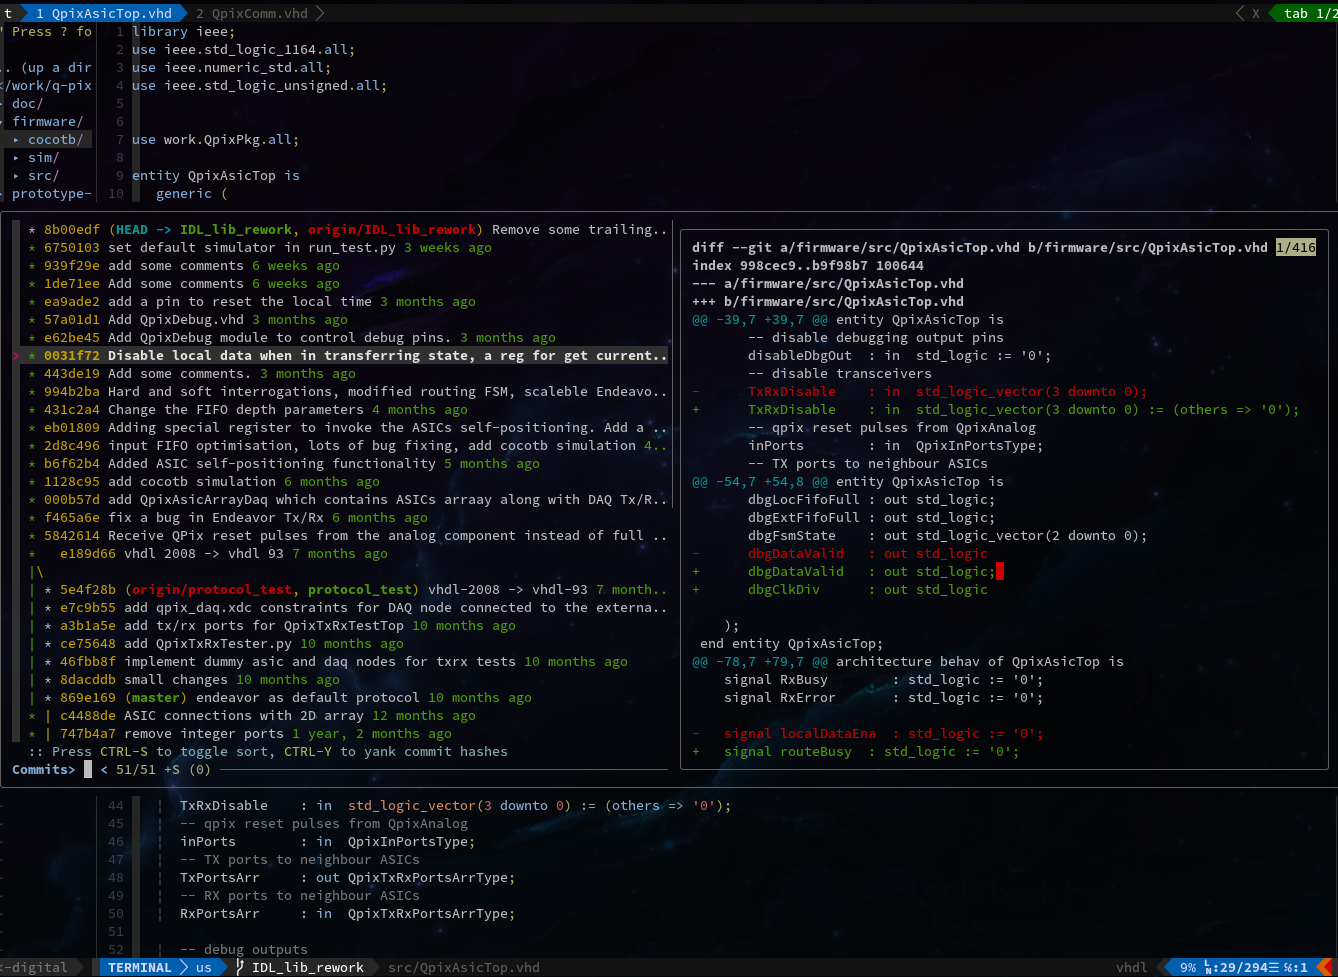
\includegraphics[width=1.0\textwidth]{figs/git_fzf_commits.png}
      
    \end{column}
  \end{columns}
  	
\end{frame}
%%%%%%%%%%%%%%%%%%%%%%%%%%%%%%%%%%%%%%%%%%%%%%%%%%%%


%%%%%%%%%%%%%%%%%%%%%%%%%%%%%%%%%%%%%%%%%%%%%%%%%%%%
\section*{Syntax checking}
%%%%%%%%%%%%%%%%%%%%%%%%%%%%%%%%%%%%%%%%%%%%%%%%%%%%
\begin{frame}{\secname}

  \begin{block}{Vim/NeoVim syntax checkers}
    Provide syntax check, autocompletion, diagnostics, go to definition, show documentation, etc.
  \begin{itemize}
    \item CoC  \\ \myurl{https://github.com/neoclide/coc.nvim} 
    \item ALE \\ \myurl{https://github.com/dense-analysis/ale}
    \item Syntastic \\ \myurl{https://github.com/vim-syntastic/syntastic}
    \item NeoVim builtin LSP
  \end{itemize}
  \end{block}

  \begin{block}{hdl$\_$checker}
    \begin{itemize}
     \item HDL language server  for VHDL/Verilog/SystemVerilog
     \item Supports Modelsim/Questa, GHDL, Vivado Simulator
     \item \myurl{https://github.com/suoto/hdl_checker}
    \end{itemize}
    
  \end{block}
    
\end{frame}
%%%%%%%%%%%%%%%%%%%%%%%%%%%%%%%%%%%%%%%%%%%%%%%%%%%%

%%%%%%%%%%%%%%%%%%%%%%%%%%%%%%%%%%%%%%%%%%%%%%%%%%%%
\section*{Snippets}
%%%%%%%%%%%%%%%%%%%%%%%%%%%%%%%%%%%%%%%%%%%%%%%%%%%%
\begin{frame}{\secname}
  \begin{block}{Vim plugins}
    \begin{itemize}
      \item Vim-snippets \myurl{https://github.com/honza/vim-snippets}
      \item Ultinsips \myurl{https://github.com/SirVer/ultisnips}
      \item Snipmate  \myurl{https://github.com/garbas/vim-snipmate}
      \item Neosnippet \myurl{https://github.com/Shougo/neosnippet.vim} 
    \end{itemize} 
  \end{block}

  \begin{block}{Templates}
    \begin{itemize}
      \item TerosHDL has templates for entity instances, testbenches, and cocotb tests.
      \item For Vim this plugin can generate entity/components instances: https://github.com/vim-scripts/VIP .
      \item There are a number of testbench generators on Github for instance: \\
        \myurl{https://github.com/phillbush/tbgen}\\
        \myurl{https://github.com/JC-LL/vhdl_tb}\\
        \myurl{https://github.com/connorcl/testbench-gen}\\
    \end{itemize}
    
  \end{block}
    
\end{frame}
%%%%%%%%%%%%%%%%%%%%%%%%%%%%%%%%%%%%%%%%%%%%%%%%%%%%

%%%%%%%%%%%%%%%%%%%%%%%%%%%%%%%%%%%%%%%%%%%%%%%%%%%%
\section*{CTags}
%%%%%%%%%%%%%%%%%%%%%%%%%%%%%%%%%%%%%%%%%%%%%%%%%%%%
\begin{frame}{\secname}
  \textbf{Ctags} is a programming tool that generates an index (or tag) file of names found in source and header files of various programming languages to aid code comprehension. (c)Wikipedia
  \begin{itemize}

    \item Exuberant ctags \myurl{https://ctags.sourceforge.net}
    \item Universal ctags \myurl{https://github.com/universal-ctags/ctags}

  \end{itemize}

  \begin{block}{Vim plugins}
    \begin{itemize}
      \item vim-tagbar \myurl{https://github.com/universal-ctags/ctags}
      \item Vista.vim \myurl{https://github.com/liuchengxu/vista.vim}
    \end{itemize} 
  \end{block}
  Fast navigation through \textit{tags} with FZF!
  	
\end{frame}
%%%%%%%%%%%%%%%%%%%%%%%%%%%%%%%%%%%%%%%%%%%%%%%%%%%%

%%%%%%%%%%%%%%%%%%%%%%%%%%%%%%%%%%%%%%%%%%%%%%%%%%%%
\section*{Git integration}
%%%%%%%%%%%%%%%%%%%%%%%%%%%%%%%%%%%%%%%%%%%%%%%%%%%%
\begin{frame}{\secname}
  \begin{columns}
    \begin{column}{0.5\textwidth}
  \begin{itemize}
    \item \myurl{https://github.com/airblade/vim-gitgutter}
      Marks modified lines of the current buffer.
    \item \myurl{https://github.com/tpope/vim-fugitive} \\ 
      \textit{``it's so awesome, it should be illegal''} \\(c) it's GitHub page.
  \end{itemize}
  Show last changes, diff with a given commit, show logs and more.
      
    \end{column}
    \begin{column}{0.6\textwidth}
      \begin{block}{Fugitive}
        \begin{tabular}{ll}
          :Git & Gives an \textbf{interactive}(!) version of the git status: \\
               & can add/reset specific file,   \\
               & open file, undo changes and everything. \\
         :Gwrite & Stage the current file to the index. \\
         :Gread  & Revert current file (git checkout). \\ 
         :Gremove & Delete the current file and vim buffer. \\
         :Gllog   & Git log. \\
         :Gvdiffsplit & Open line by line diff in a vertical split.

        \end{tabular}
        
      \end{block} 
    \end{column}
  \end{columns}
    
\end{frame}
%%%%%%%%%%%%%%%%%%%%%%%%%%%%%%%%%%%%%%%%%%%%%%%%%%%%

%%%%%%%%%%%%%%%%%%%%%%%%%%%%%%%%%%%%%%%%%%%%%%%%%%%%
\section*{Integration with terminal}
%%%%%%%%%%%%%%%%%%%%%%%%%%%%%%%%%%%%%%%%%%%%%%%%%%%%
\begin{frame}[fragile]{\secname}
  \begin{block}{Vim}
    \begin{itemize}
      \item :terminal -- open built-in terminal
      \item !command  -- execute command and put output into the quickfix window
      \item \lstinline{:new | r ! command} -- execute command and put output into a new buffer
      \item AsyncRun -- {\color{blue} \myurl{https://github.com/skywind3000/asyncrun.vim}} \\
        Run shell comand in the background.  E.g. : \\
        \lstinline{:AsyncRun make} -- do make in the background. \\
        \lstinline{:AsyncRun git push} -- git push.\\
        \lstinline{:AsyncRun -mode=term -pos=tab ./% } -- run current buffer and show output in the new tab\\
     \lstinline{:AsyncRun -mode=term -pos=right ./% } -- run current buffer and show output on the right split\\
    \end{itemize}
  \end{block}	
  \begin{block}{VSCode}
    \begin{itemize}
      \item VSCode has a built-in terminal window.
      \item Can run commands asynchronously as well.
    \end{itemize}
    
  \end{block}
\end{frame}
%%%%%%%%%%%%%%%%%%%%%%%%%%%%%%%%%%%%%%%%%%%%%%%%%%%%

%%%%%%%%%%%%%%%%%%%%%%%%%%%%%%%%%%%%%%%%%%%%%%%%%%%%
\section*{TerosHDL amazing features}
%%%%%%%%%%%%%%%%%%%%%%%%%%%%%%%%%%%%%%%%%%%%%%%%%%%%
\begin{frame}{\secname}

  See \myurl{https://terostechnology.github.io/terosHDLdoc/} for the full list of features
  with gif previews.

  \begin{itemize}
    \item State machine viewer
    \item Templates : components/entities/testbenches/cocotb
    \item Hierarchy view/dependencies graph
    \item Schematic viewer (synthesis with YoSys)
    \item Automatic documentation (with wavedrom/bitfield integration) \\
      Wavedrom (\myurl{https://wavedrom.com}) is a powerful tool to draw timing diagrams.\\
      It has online editor: \myurl{https://wavedrom.com/editor.html}.
    \item Integration with Modelsim, Quartus, Vivado, Radiant, and everything.
  \end{itemize}
    
\end{frame}
%%%%%%%%%%%%%%%%%%%%%%%%%%%%%%%%%%%%%%%%%%%%%%%%%%%%

%%%%%%%%%%%%%%%%%%%%%%%%%%%%%%%%%%%%%%%%%%%%%%%%%%%%
\section*{Some links}
%%%%%%%%%%%%%%%%%%%%%%%%%%%%%%%%%%%%%%%%%%%%%%%%%%%%
\begin{frame}{\secname}
  \begin{block}{Vim}
    \begin{itemize}
      \item \myurl{https://www.vim.org/}
      \item \myurl{https://vimawesome.com/}
      \item Introduction to Vim in Russian \myurl{https://www.youtube.com/watch?v=jkxLIFVGfd4}
    \end{itemize}
  \end{block}

  \begin{block}{VsCode}
    \begin{itemize}
      \item \myurl{https://www.youtube.com/@terostechnology5520}
      \item Presentation ``TerosHDL: an open source IDE for FPGA developers'' \myurl{https://www.youtube.com/watch?v=_wxTjOSO5oY}
    \end{itemize}
  \end{block}
  	
\end{frame}
%%%%%%%%%%%%%%%%%%%%%%%%%%%%%%%%%%%%%%%%%%%%%%%%%%%%


\end{document}




